\documentclass{beamer}
\usetheme{Madrid}
\usecolortheme{whale}
%\usepackage{graphicx}
%\graphicspath{{img/}}
\usepackage[utf8]{inputenc}
\usepackage{graphicx}
\usepackage[spanish]{babel}
\usepackage{booktabs}
\usepackage{color}

\title[Regresión Lineal]{Fundamentos de la Programación Estadística en R}
\subtitle{Algunas nociones fundamentales de Machine Learning}
\author{Germán Rosati \\ \href{ german.rosati@gmail.com}{german.rosati@gmail.com}}
\institute{UNTREF - UNSAM - Digital House}
\date{12 de Marzo de 2018}
%\logo{\includegraphics[height=0.4cm]{img/header-logo.png}}

\begin{document}
\frame{\titlepage}
%\begin{frame}
%	\frametitle{Hoja de ruta}
%	\tableofcontents
%\end{frame}

\section{¿Qué es un modelo?}
\begin{frame}
\frametitle{¿Qué es un modelo?}
	\begin{itemize}
		\item{Básicamente: una manera de proponer hipótesis sobre la forma en que se combinan variables}
		\item{En general, vamos a estar tratando de generar modelos de esta forma 
			\begin{equation}
				Y = f(X) + \epsilon
			\end{equation}}
		\item{Todo el problema es estimar $f(X)$, es decir, de qué forma(s) se combinan las $X$ para generar un output}
		\item{Una posibilidad es suponer que $Y$ es una combinación lineal de las $X$}
	\end{itemize}
\end{frame}


\subsection{Debates sobre el modelado}
\begin{frame}
	\frametitle{¿Qué es un modelo?}
	\framesubtitle{Las dos culturas (Breiman, 2001)}
	\begin{quotation}
		``Todos los modelos son equivocados. Algunos son útiles.''\\ George Box
	\end{quotation}
	\begin{itemize}
		\item{Podemos pensar al mundo como un productor de outputs en base a features}
		
		\begin{figure}
			\centering
			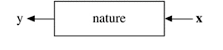
\includegraphics[width=0.5\linewidth, height=0.15\textheight]{img/two_cult_nature}
		\end{figure}
		
		\item{Caja negra en las que se combinan las $X$ de alguna forma que desconocemos}
		\item{Los problemas surgen cuando queremos estimar cuál es la manera en que el mundo produce resultados}
	\end{itemize}
\end{frame}

\begin{frame}
	\frametitle{¿Qué es un modelo?}
	\framesubtitle{Las dos culturas (Breiman, 2001)}
	\textbf{Modelado estadístico}
	\begin{itemize}
		\item{Se comienza asumiendo que dentro de la caja negra hay un modelo estadístico}
		\item{Una forma común es asumir que los datos son generados por extracciones independientes de $output = f(predictores, ruido, parametros)$}
		\item{Los parámetros son estimados con los datos y luego se realizan las predicciones. La caja se llena con}
		\begin{figure}
			\centering
			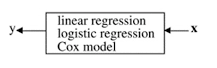
\includegraphics[width=0.55\linewidth, height=0.18\textheight]{img/two_cult_stat}
		\end{figure}
		\item{Validación: Sí-No, usando medidas de bondad de ajuste y análisis de residuos}		
	\end{itemize}
\end{frame}

\begin{frame}
	\frametitle{¿Qué es un modelo?}
	\framesubtitle{Las dos culturas (Breiman, 2001)}
	\textbf{Modelado algorítmico (o \emph{Machine Learning}, \emph{Data Mining}, etc.)}
	\begin{itemize}
		\item{Se comienza asumiendo lo que pasa dentro de la caja es demasiado complejo y desconocido}
		\item{El enfoque es encontrar una función $f(x)$ -un algoritmo- que opera sobre las $x$ para predecir las $y$. La caja negra tiene esta forma}
		\begin{figure}
			\centering
			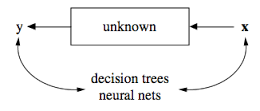
\includegraphics[width=0.55\linewidth, height=0.25\textheight]{img/two_cult_algoritmic}
		\end{figure}
		\item{Validación: medido a través de la cuantificación de la precisión predictiva}		
	\end{itemize}
\end{frame}

\subsection{¿Cómo evaluar un modelo?}
\begin{frame}
	\frametitle{¿Qué es un modelo?}
	\framesubtitle{¿Cómo evaluar un modelo?}
	\begin{itemize}
		\item{Ahora bien, ¿qué es un buen modelo?}
		\item{Desde la cultura del \textbf{modelado estadístico} un buen modelo es un modelo que ajusta bien a los datos y cuyos parámetros cumplen algunas propiedades ``deseables''}
		\begin{enumerate}
			\item Ser insesgado
			\item Ser robusto 
			\item Tener varianza mínima...
			\item Etc...			
		\end{enumerate}
	\end{itemize}
\end{frame}

\begin{frame}
	\frametitle{¿Qué es un modelo?}
	\framesubtitle{¿Cómo evaluar un modelo?}
	\begin{itemize}
		\item{El \textbf{modelado algorítimo} piensa sobre todo en la capacidad predictiva}
		\item{Pero... ¿sobre cuáles datos?}
		\item{Queremos modelos que funcionen bien -tengan bajo error- en datos que NO vimos, es decir, en datos ``futuros'', datos de test, \emph{out of sample}}
		\item{Pero muchas veces esos datos no existen o tardan en aparecer}
		\item{$\implies$ Separación en \emph{Training Data} y \emph{Test Data}}
		\item{Entreno-estimo-construyo el modelo sobre \emph{Training Data} y evalúo sobre \emph{Test Data}}
	\end{itemize}
\end{frame}


\begin{frame}
	\frametitle{¿Qué es un modelo?}
	\framesubtitle{¿Cómo evaluar un modelo?}
	\begin{itemize}
		\item{Que un modelo funcione bien en datos de entrenamiento no quiere decir que funcione bien en datos nuevos...}
		\item{En general, el error en datos de entrenamiento es más bajo que el error en datos de test}
	\end{itemize}
\end{frame}

\begin{frame}
	\frametitle{¿Qué es un modelo?}
	\framesubtitle{¿Cómo evaluar un modelo?}
	\begin{itemize}
		\color{red}
		\item{Función original: $f(x_{i})=500+0.4X_{i}^3+\epsilon_{i}$}
		\color{orange}
		\item{Modelo Lineal: $\hat{f}(x_{i})=\hat{\beta_{0}}+\hat{\beta_{1}}X_{i}$}
		\color{blue}
		\item{Modelo Cuadrático: $\hat{f}(x_{i})=\hat{\beta_{0}}+\hat{\beta_{1}}X_{i}+\hat{\beta_{2}}X_{i}^2$}
		\color{green}
		\item{Modelo Polinómico de orden 25: $\hat{f}(x_{i})=\hat{\beta_{0}}+\hat{\beta_{1}}X_{i}+\hat{\beta_{2}}X_{i}^2+...++\hat{\beta_{25}}X_{i}^{25}$}
	\end{itemize}
\end{frame}

\begin{frame}
	\frametitle{¿Qué es un modelo?}
	\framesubtitle{¿Cómo evaluar un modelo?}
	\begin{figure}
		\centering
		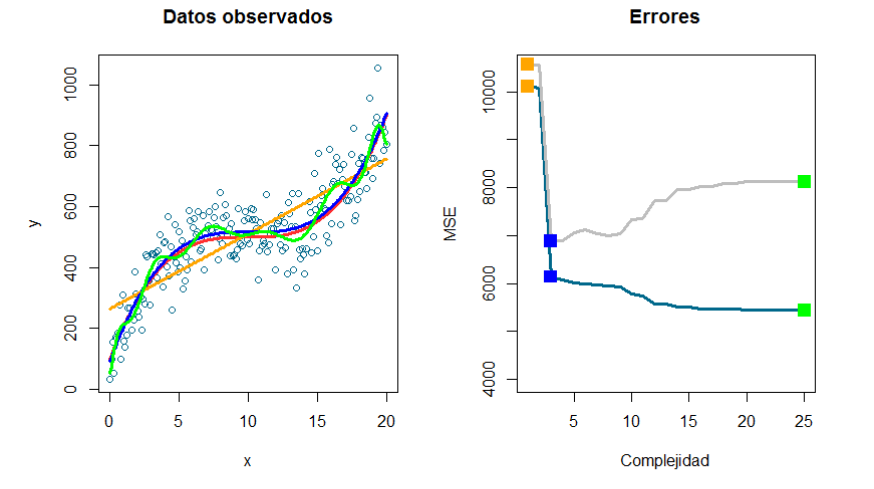
\includegraphics[width=0.9\linewidth, height=0.7\textheight]{img/train_test_error}
	\end{figure}
\end{frame}

\begin{frame}
	\frametitle{¿Qué es un modelo?}	
	\framesubtitle{¿Cómo evaluar un modelo?}
	\begin{itemize}
		\item{TrS-error decrece constantemente: siempre es posible generar un modelo muy “complejo” como para que ajuste bien a los datos (¿cuáles?)}
		\item{TeS-error decrece hasta un punto y 	luego comienza a crecer nuevamente. Se produce “overfitting” (sobreajuste).}
		\item{El modelo “trabaja” demasiado para 		encontrar patrones en el TrS y tiende a confundir el verdadero patrón ($f(x)$ - el “proceso generador de los datos”) con ruido ($\epsilon$) que no existe en el TeS.}
	\end{itemize}
\end{frame}

\begin{frame}
	\frametitle{¿Qué es un modelo?}
	\framesubtitle{¿Cómo evaluar un modelo? - Balance Sesgo-Varianza}
	\begin{itemize}
		\item{El ECM puede descomponerse en tres partes}
		\begin{equation}
		E[(y - \hat{f}(x))^2]=V(\hat{f}(x)) + bias^2 +\sigma^2
		\end{equation}	
		\item{Error debido al sesgo: diferencia entre el valor esperado de nuestra predicción y el verdadero valor poblacional}
		\item{Error debido a la varianza: producido por la variabilidad de las predicciones del modelo en un punto determinado.}
		\item{El $\sigma^2$ es la parte "irreductible" del error en el modelo}
	\end{itemize}
\end{frame}

\begin{frame}
	\frametitle{¿Qué es un modelo?}
	\framesubtitle{¿Cómo evaluar un modelo? - Algunos trade-offs}
	\begin{figure}
		\centering
		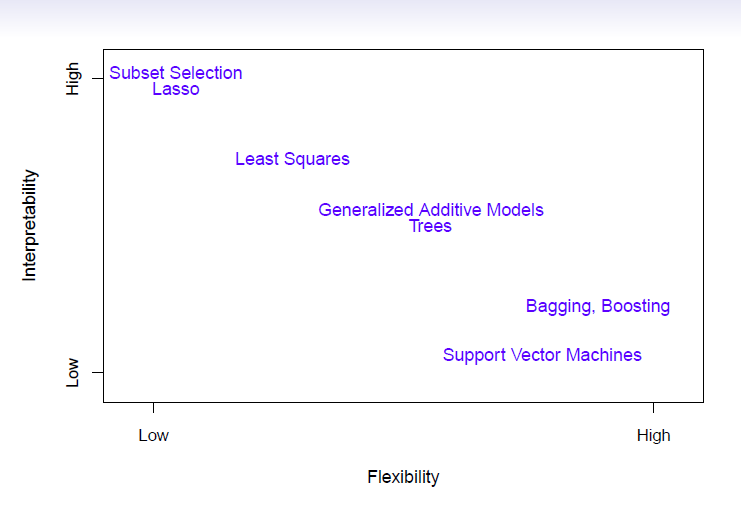
\includegraphics[width=0.7\linewidth, height=0.7\textheight]{img/trade_offs}
	\end{figure}
	{\footnotesize\textbf{Fuente:} James, Witten, Hastie y Tibshiraini (2013): 25}
\end{frame}

\begin{frame}
	\frametitle{¿Qué es un modelo?}
	\framesubtitle{¿Cómo evaluar un modelo? - Balance Sesgo-Varianza}
	\begin{figure}
		\centering
		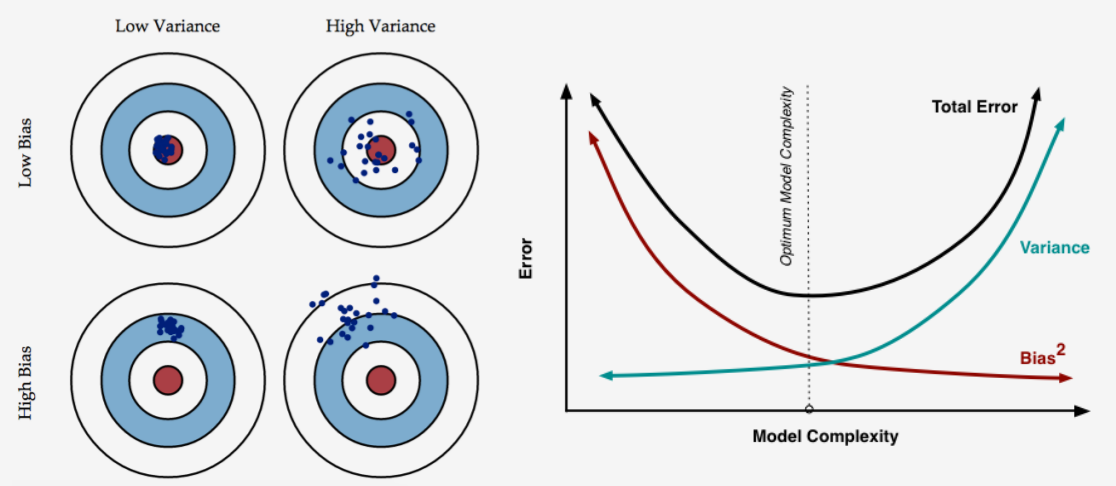
\includegraphics[width=0.8\linewidth, height=0.5\textheight]{img/bias_variance}
	\end{figure}
\end{frame}

\begin{frame}
	\frametitle{¿Qué es un modelo?}
	\framesubtitle{¿Cómo evaluar un modelo?}
	\begin{itemize}
		\item{Herramientas para estimar el error de generalización de un modelo -qué tan bien va a funcionar sobre datos ``no vistos''}
		\begin{enumerate}
			\item{\emph{Validation Set Approach}}
			\item{\emph{Cross Validation}}
			\item{\emph{Bootsrap}}
			\item{\emph{Etc.}}
		\end{enumerate}
	\end{itemize}
\end{frame}

\begin{frame}
	\frametitle{¿Qué es un modelo?}
	\framesubtitle{Validation Set Approach}
	\begin{itemize}
		\item{Dividimos el \textbf{aleatoriamente} \emph{dataset} en \emph{Training Set - TrS} y \emph{Test Set - TeS}}
		\item{El modelo se ajusta en el TrS y el modelo ajustado se usa para predecir las observaciones correspondientes al TeS}
	\end{itemize}
\end{frame}

\begin{frame}
	\frametitle{¿Qué es un modelo?}
	\framesubtitle{Cross Validation}
	\begin{itemize}
		\item{Dividimos el \textbf{aleatoriamente} \emph{dataset} en $K$ porciones de igual tamaño}
		\item{Fiteamos el modelo dejando como TeS una de las $K$ partes}
		\item{Computamos el error en la parte dejada afuera previamente}
		\item{Repetimos para $k=1,2,3,...,K$}
		\item{La estimación del error será el promedio de las $K$ estimaciones de error}
	\end{itemize}
\end{frame}

\begin{frame}
	\frametitle{¿Qué es un modelo?)}
	\framesubtitle{Cross Validation}
	\begin{figure}
		\centering
		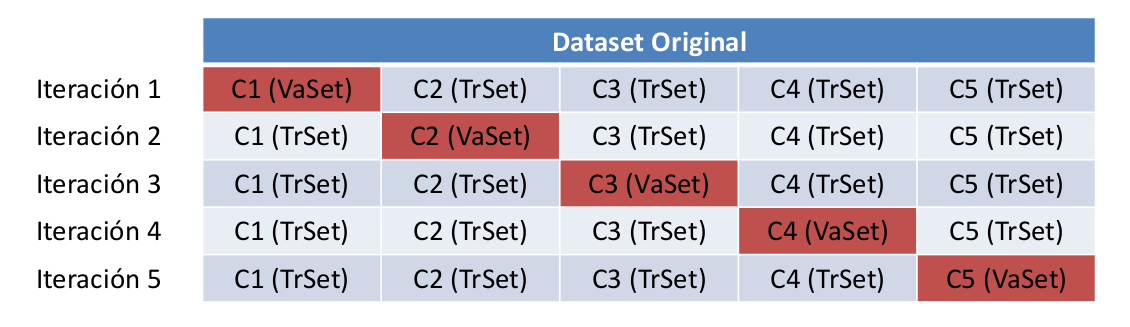
\includegraphics[width=0.9\linewidth, height=0.5\textheight]{img/cv}
	\end{figure}
\end{frame}


\section{Comentarios finales}
\begin{frame}
	\frametitle{Comentarios finales}
	\begin{itemize}
		\item{La máxima de Box...}
		\item{Dado que todos los modelos son simplificaciones de la realidad, no podemos llegar a la ``verdad'' por complejidad creciente.}
		\item{Principio de Occam, caso contrario, \emph{overfitting}}
		\item{¿Modelado estadístico o algorítmico? Dependerá del problema en cuestión}
	\end{itemize}
\end{frame}

\begin{frame}
	\frametitle{Bibliografía recomendada}
	\begin{figure}
		\centering
		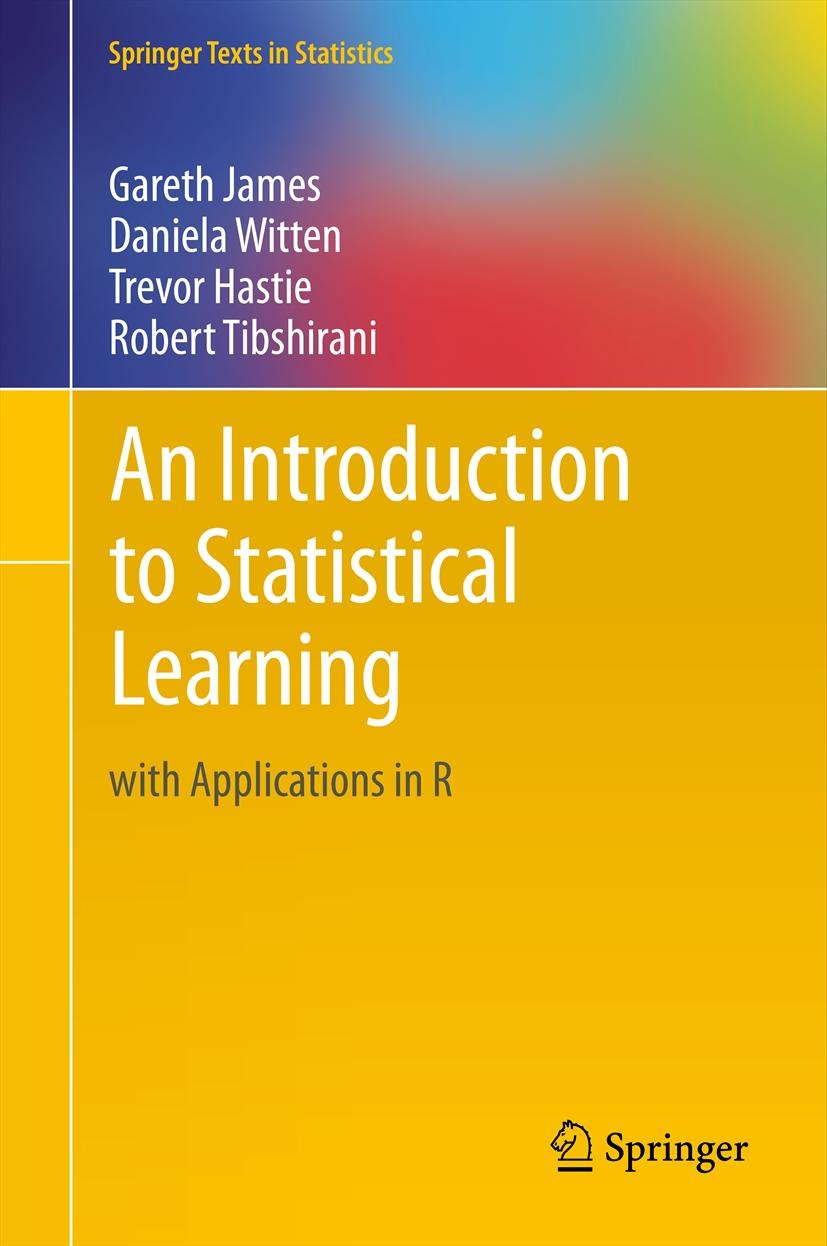
\includegraphics[width=0.33\linewidth, height=0.7\textheight]{img/ISL} 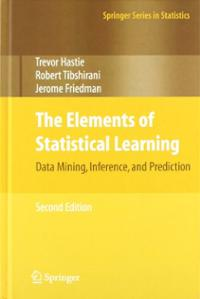
\includegraphics[width=0.34\linewidth, height=0.7\textheight]{img/ESL}
%		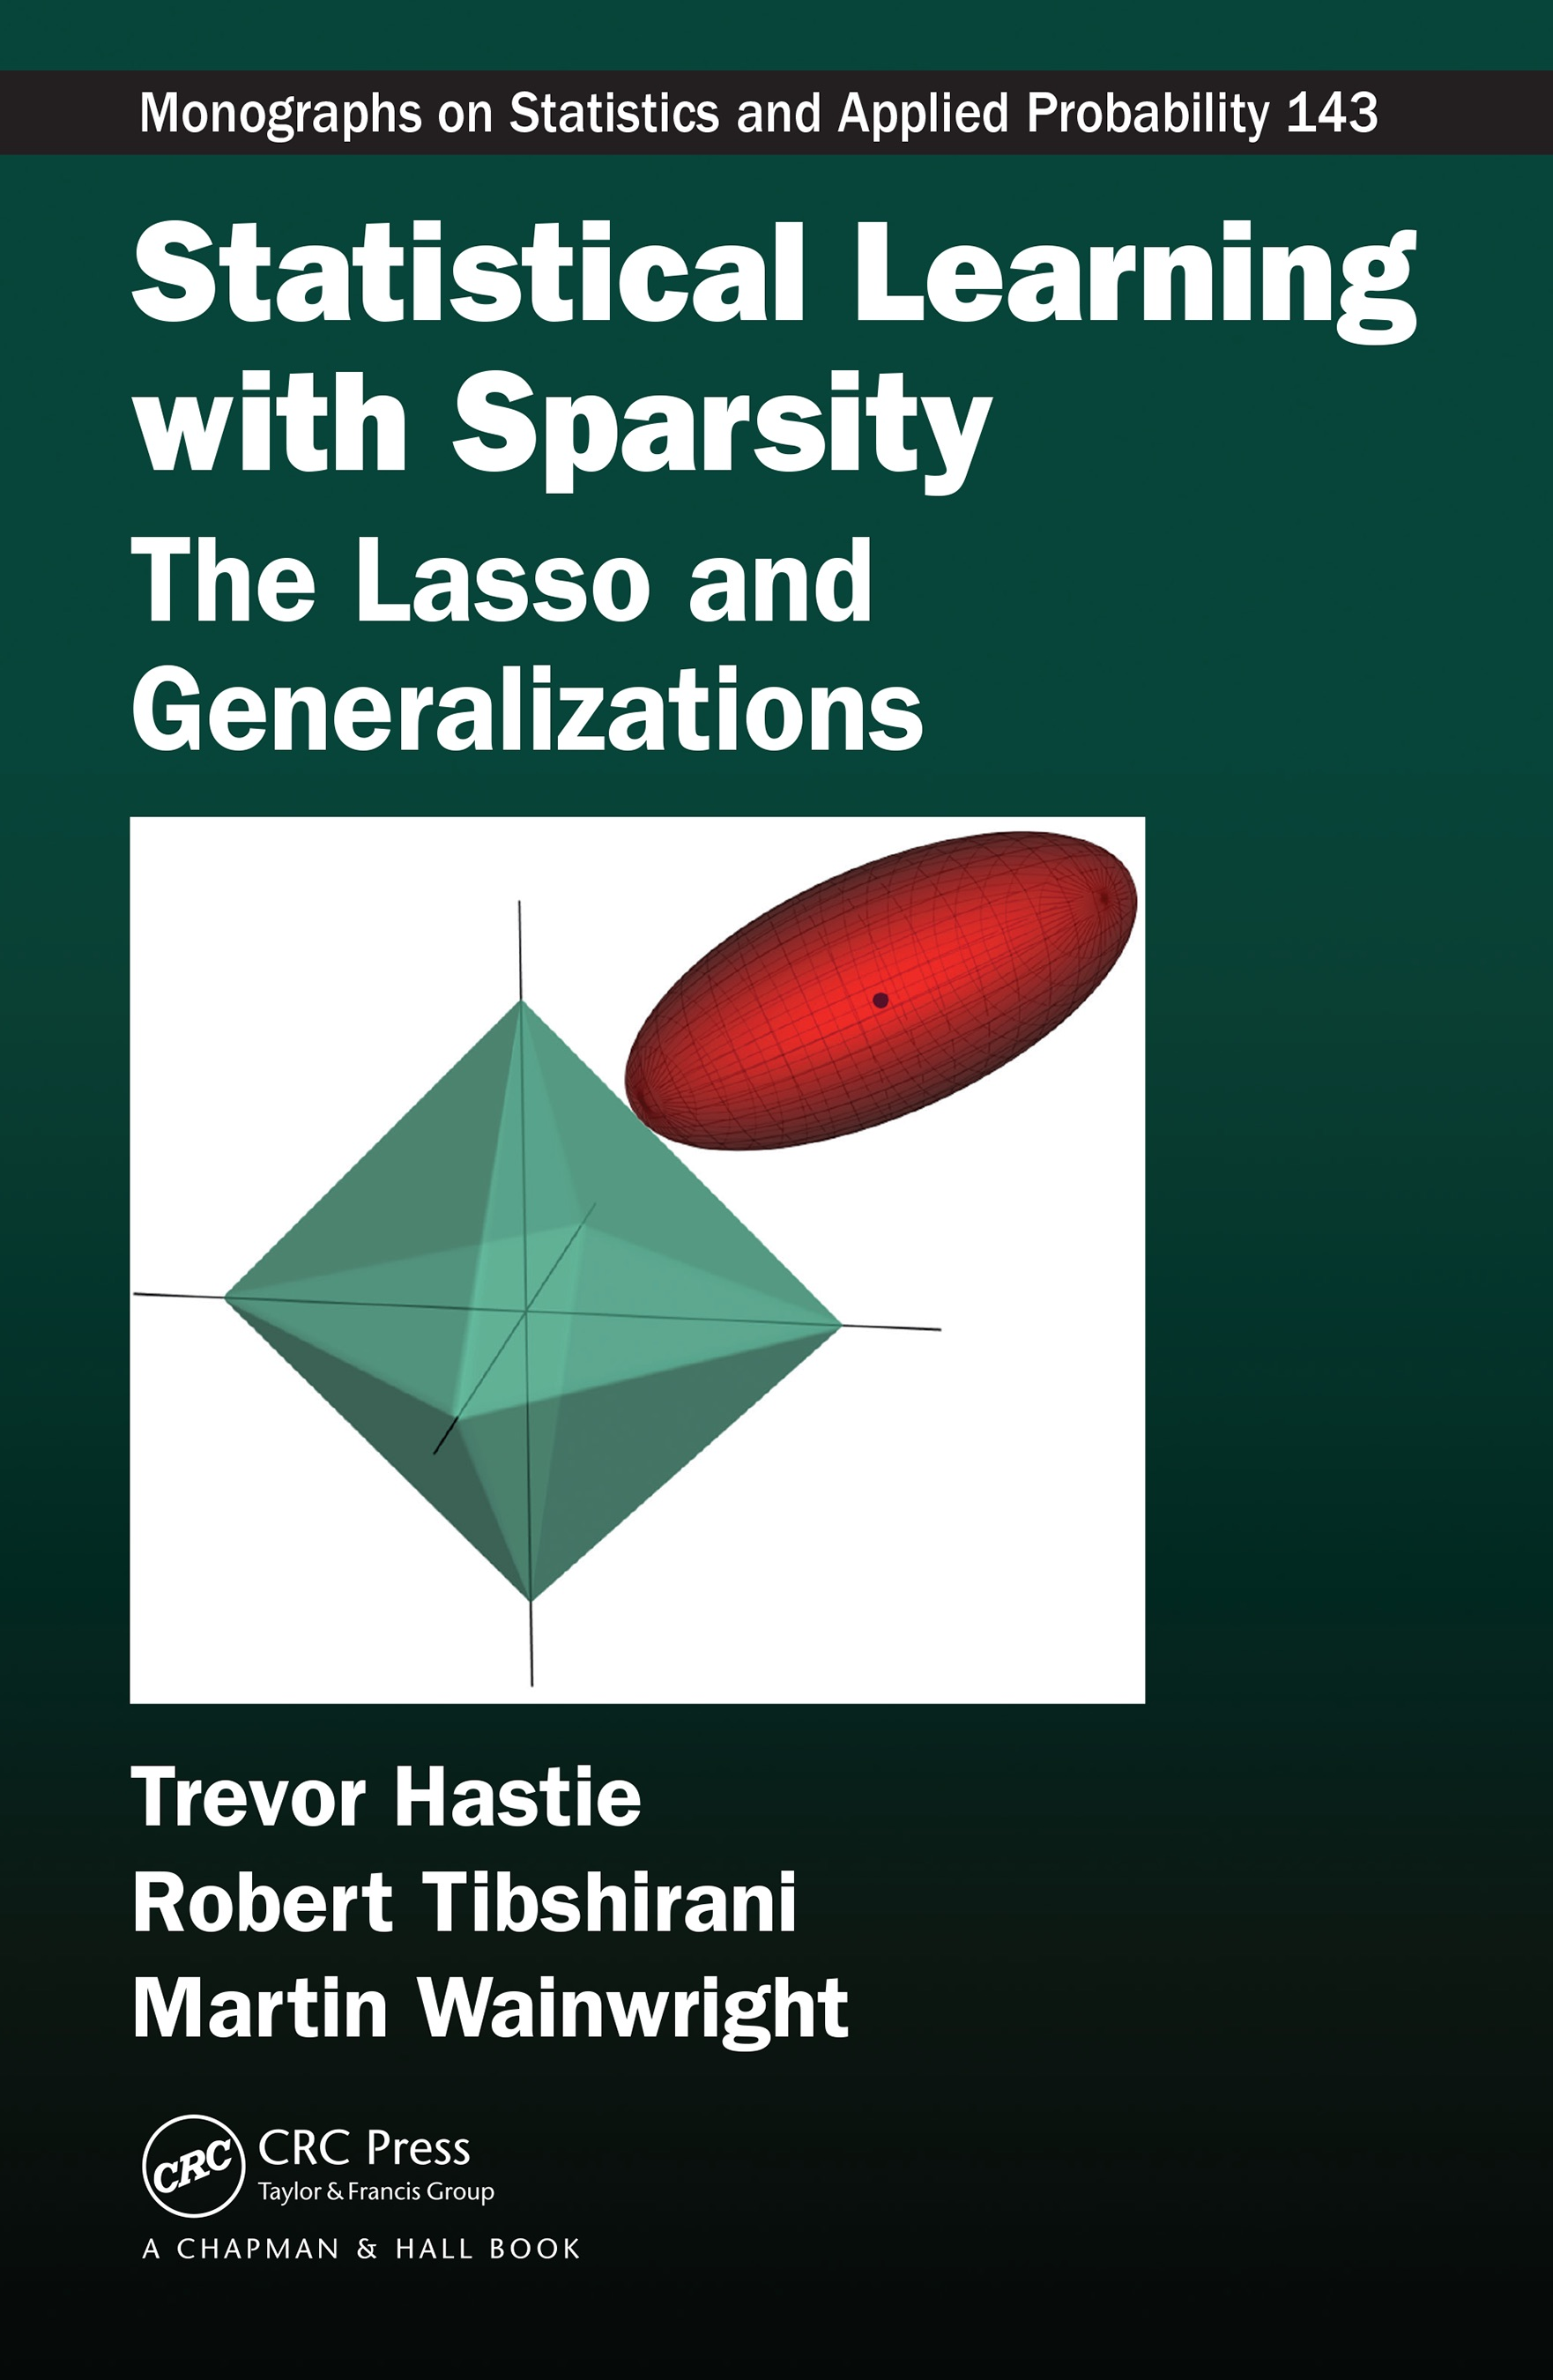
\includegraphics[width=0.34\linewidth, height=0.7\textheight]{img/sls}
	\end{figure}
\end{frame}

\end{document}